\documentclass[12pt]{article}
\usepackage[a4paper,margin=1in]{geometry}
\usepackage{iftex}
\ifPDFTeX
\usepackage[T1]{fontenc}
\usepackage[utf8]{inputenc}
\usepackage{times}
\else
\usepackage{fontspec}
\setmainfont{Times New Roman}
\fi
\usepackage{setspace}
\onehalfspacing
\usepackage{graphicx}
\usepackage{float}
\usepackage{booktabs}
\usepackage{array}
\usepackage{caption}
\usepackage{hyperref}
\usepackage{xcolor}

\newcommand{\safeincludegraphics}[2][]{%
    \IfFileExists{#2}{\includegraphics[#1]{#2}}{%
        \fbox{\parbox[c][0.18\textheight][c]{0.45\linewidth}{\centering Missing figure}}%
    }%
}

\title{CS-4063 Natural Language Processing\\Assignment 2 Report}
\author{i23-2538}
\date{April 2026}

\begin{document}
\maketitle

\noindent\textbf{GitHub URL:} \url{https://github.com/Hirotaka-Akihiro/i23-2538-NLP-Assignment}

\section*{Overview}
This report presents a complete neural NLP pipeline implemented from scratch in PyTorch for BBC Urdu-style text processing.
The assignment is divided into three parts: word representation learning, sequence labeling, and topic classification.
Part 1 includes TF-IDF, PPMI, and Skip-gram Word2Vec evaluation.
Part 2 covers POS tagging and NER using a 2-layer BiLSTM, including CRF decoding and ablations.
Part 3 implements a custom Transformer encoder for 5-class document classification and compares it to a BiLSTM baseline.
All figures and metrics are generated from the submitted notebook outputs.
The compiled report is formatted to remain within the required 2--3 page limit (target: 3 pages).

\section*{Part 1 Results: Word Embeddings}
A capped vocabulary was used to construct the term-document matrix and compute TF-IDF values.
Topic-wise top-10 discriminative terms were extracted from mean TF-IDF scores.
A symmetric co-occurrence matrix with window size $k=5$ was transformed into PPMI vectors.
The t-SNE projection for the 200 most frequent tokens is shown in Figure~\ref{fig:tsne}.

\begin{figure}[H]
    \centering
    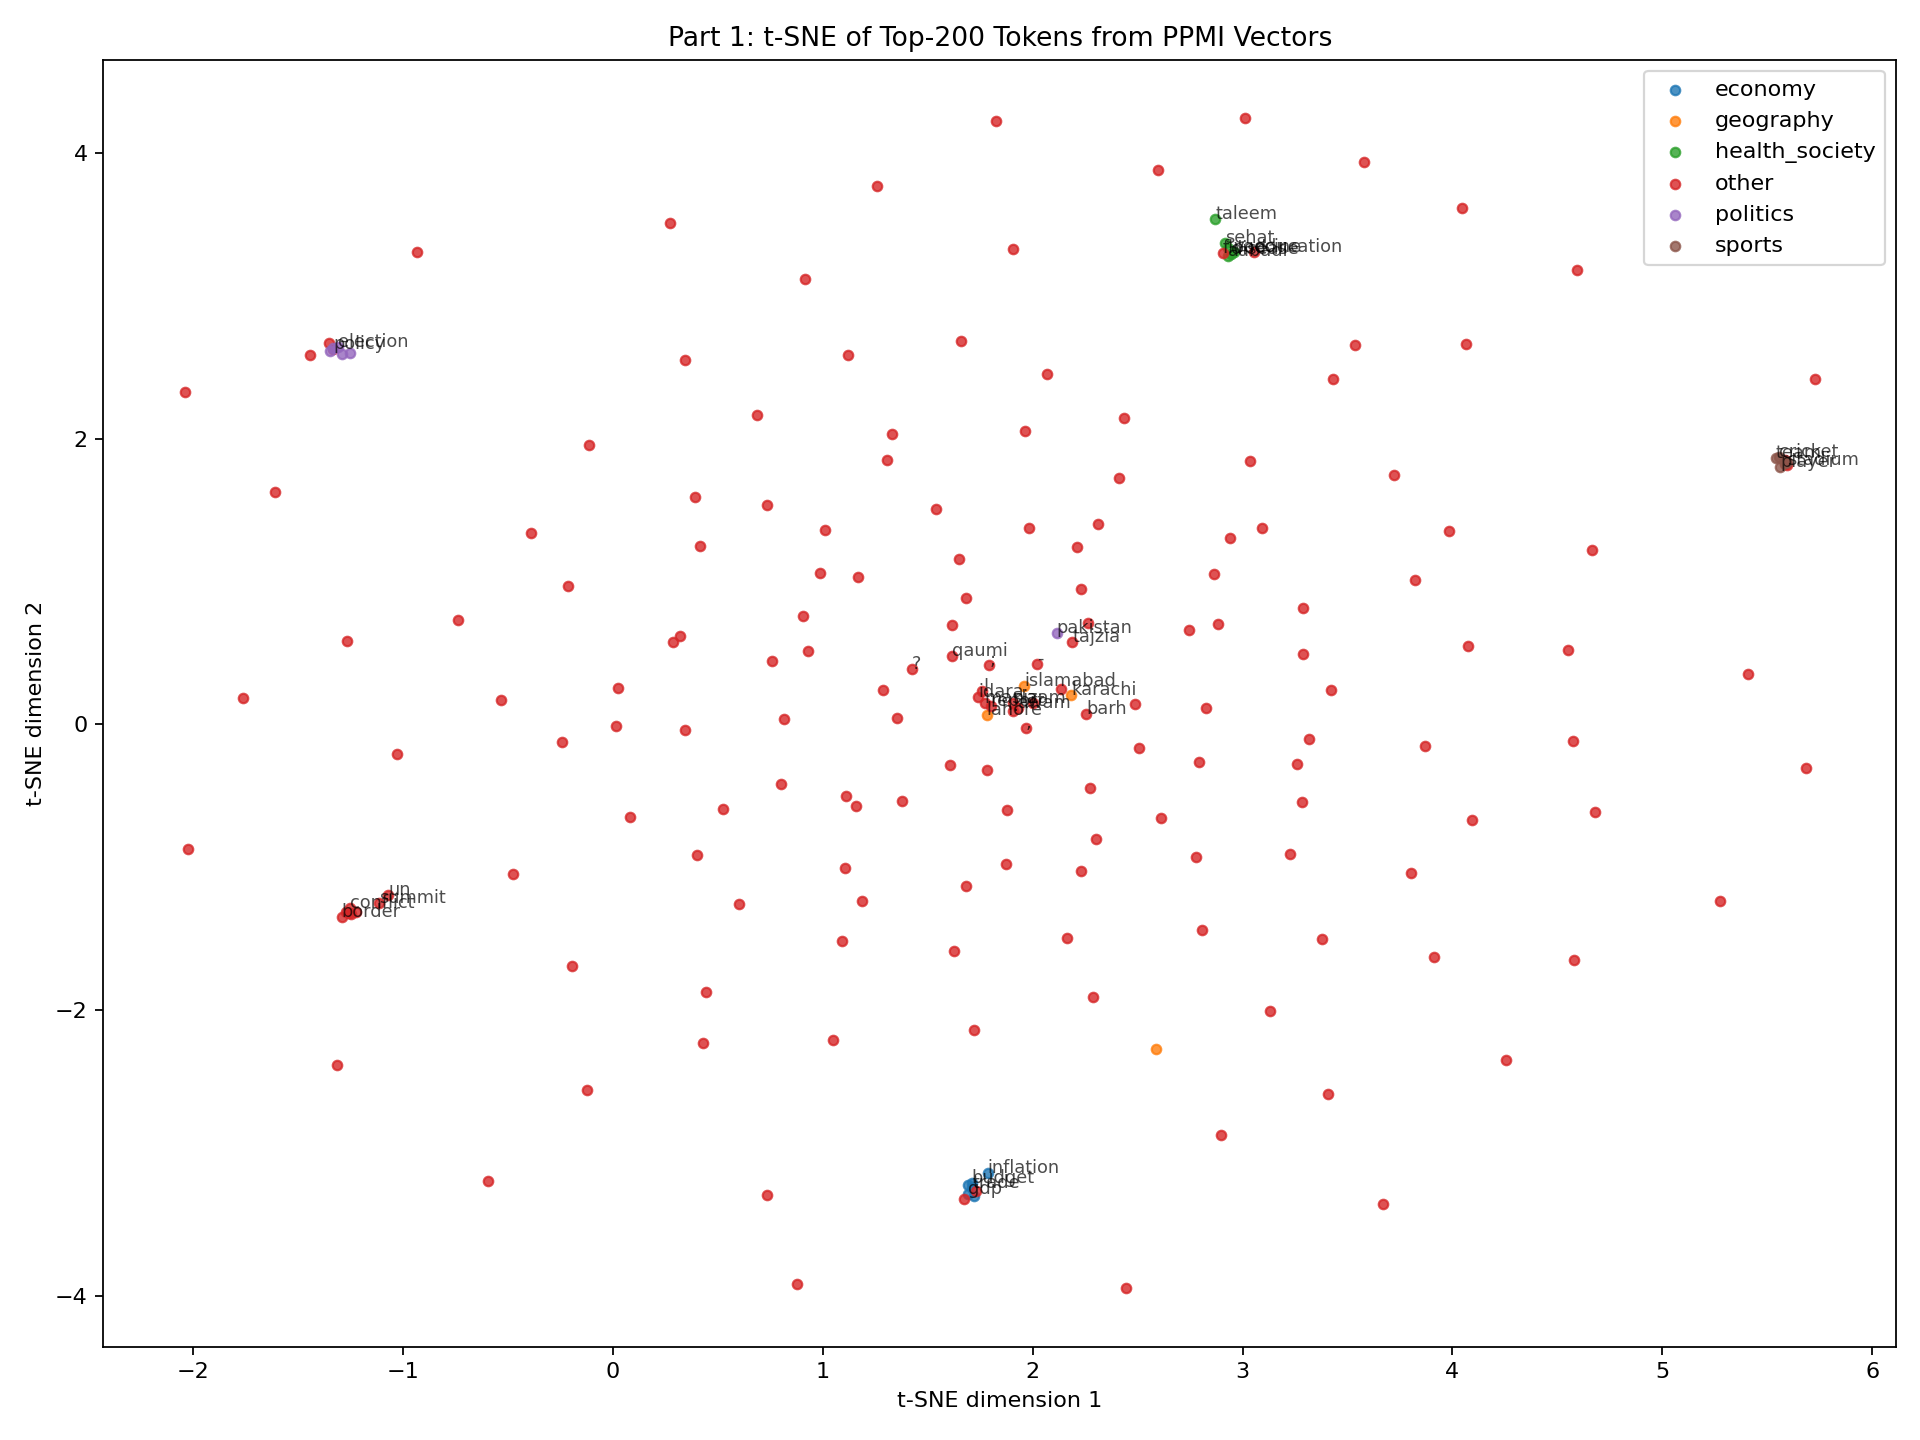
\includegraphics[width=0.9\linewidth]{Images to add/part1_ppmi_tsne.png}
    \caption{t-SNE visualization of top-200 token PPMI vectors.}
    \label{fig:tsne}
\end{figure}

The Skip-gram model (two embedding matrices, negative sampling, BCE objective) converged rapidly and stabilized after early epochs.

\begin{figure}[H]
    \centering
    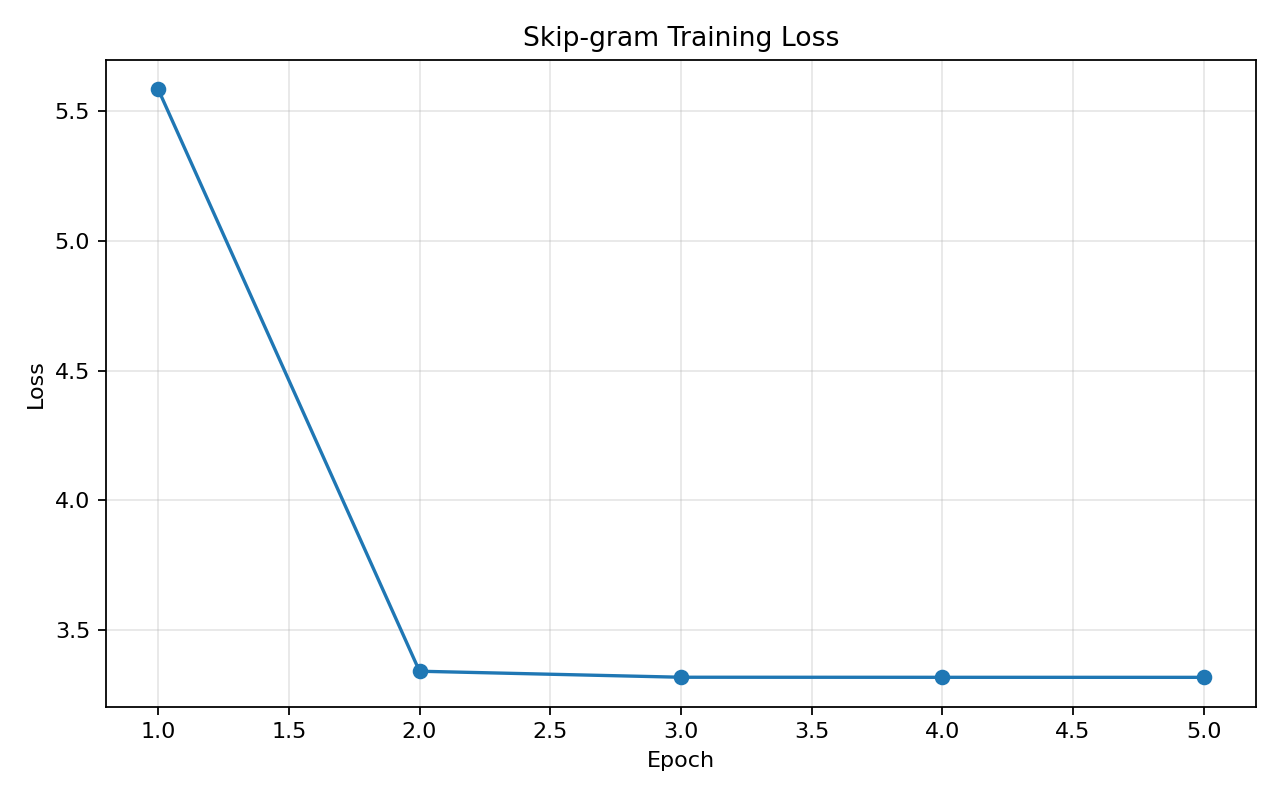
\includegraphics[width=0.72\linewidth]{Images to add/part1_skipgram_loss.png}
    \caption{Skip-gram training loss across epochs.}
    \label{fig:w2v_loss}
\end{figure}

Nearest-neighbour queries indicated coherent lexical neighborhoods for key words such as Pakistan, Hukumat, and Sehat.
Analogy tests were executed for 10 prompts with top-3 candidates reported.
The four-condition comparison (C1--C4) was performed and MRR values are summarized in Table~\ref{tab:mrr}.

\begin{table}[H]
\centering
\caption{Four-condition embedding comparison with MRR}
\label{tab:mrr}
\begin{tabular}{lll}
\toprule
Condition & Description & MRR \\
\midrule
C1 & PPMI baseline & 1.0000 \\
C2 & Skip-gram on raw corpus & 0.1333 \\
C3 & Skip-gram on cleaned corpus & 0.1000 \\
C4 & Skip-gram on cleaned corpus ($d=200$) & 0.0125 \\
\bottomrule
\end{tabular}
\end{table}

\section*{Part 2 Results: Sequence Labeling (POS + NER)}
A dataset of 500 sentences was prepared and split into train/validation/test with stratification by topic.
The BiLSTM sequence labeler was evaluated with frozen and fine-tuned embeddings.
Training curves for POS and NER are shown in Figure~\ref{fig:part2_curves}.

\begin{figure}[H]
    \centering
    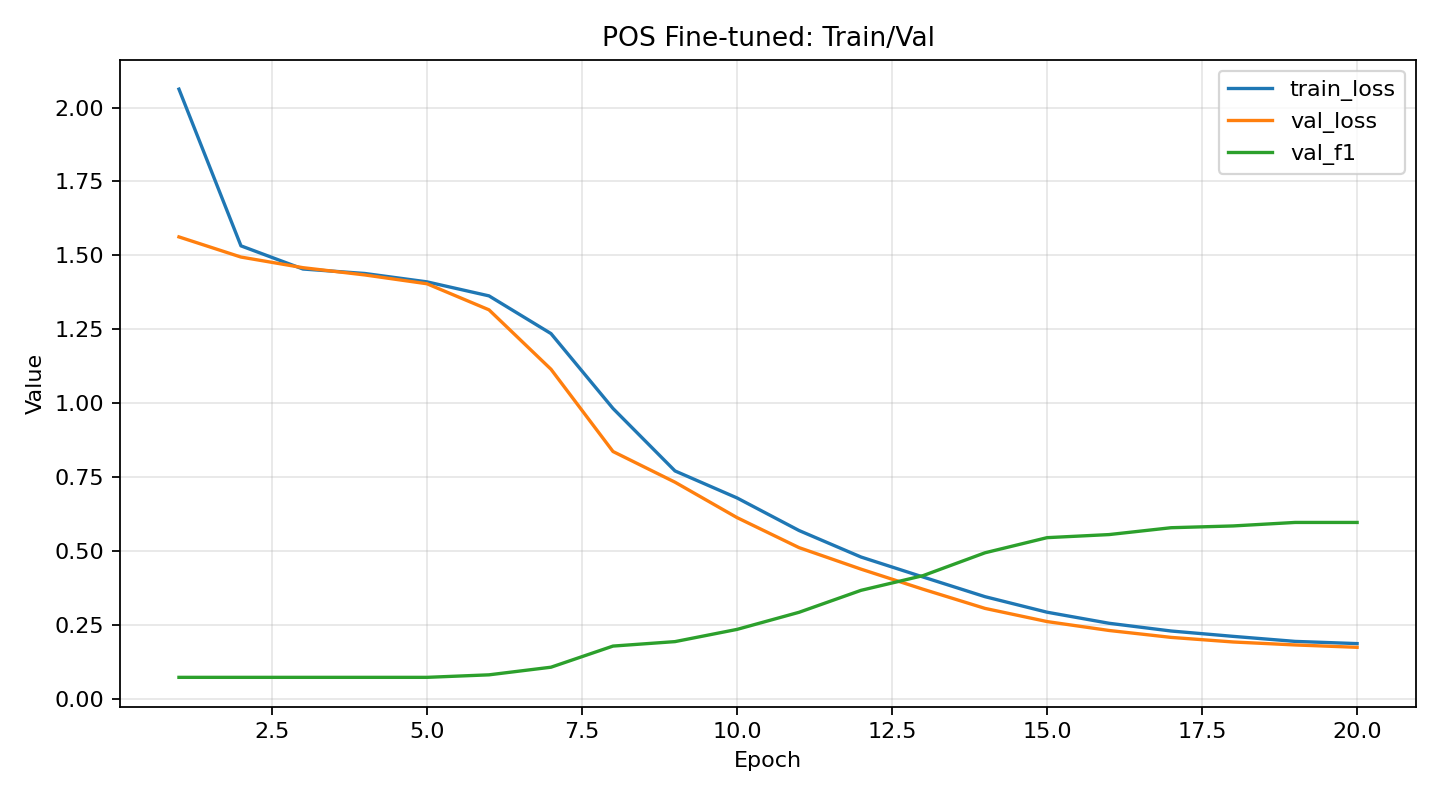
\includegraphics[width=0.48\linewidth]{Images to add/part2_pos_finetuned_curve.png}
    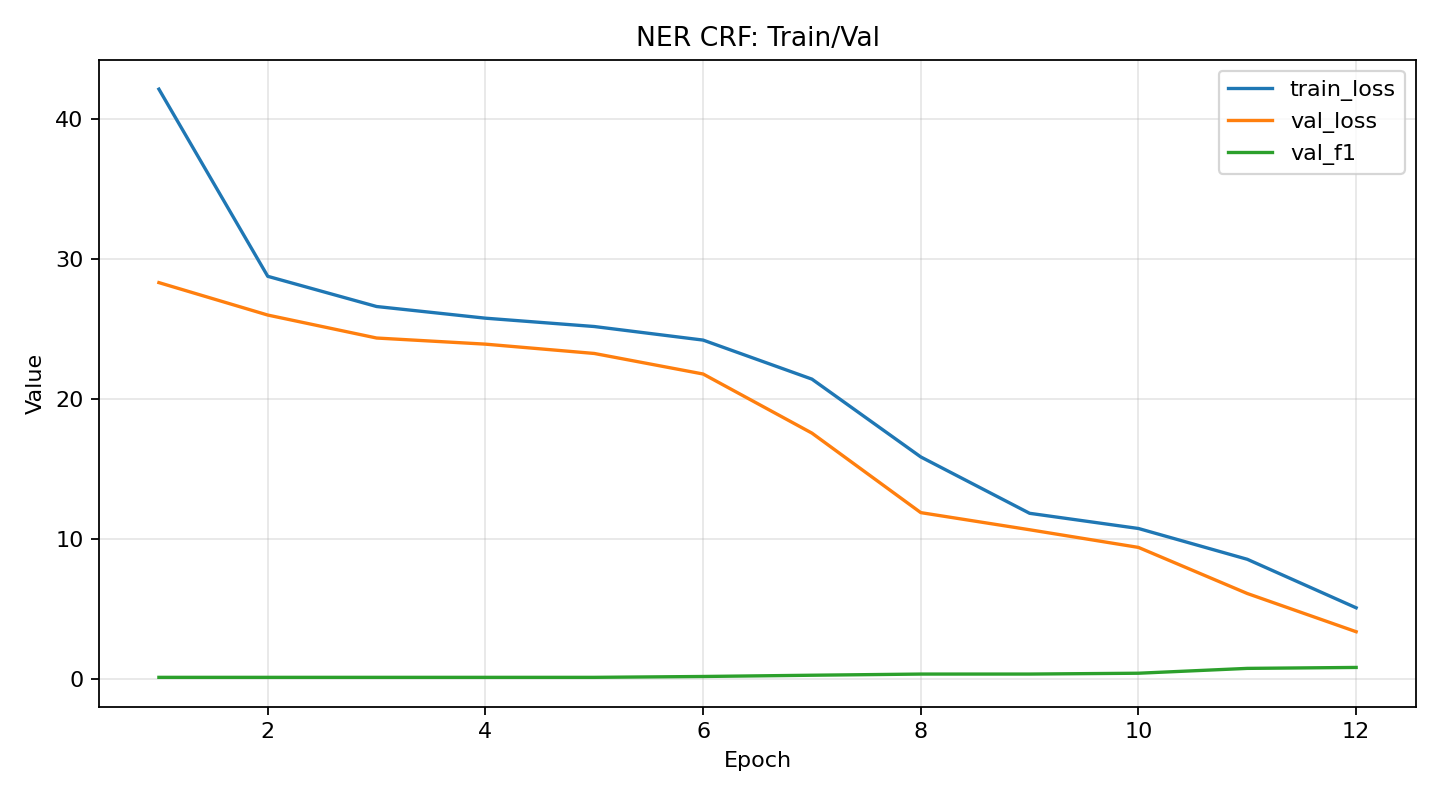
\includegraphics[width=0.48\linewidth]{Images to add/part2_ner_crf_curve.png}
    \caption{Representative training/validation curves for POS (fine-tuned) and NER (CRF).}
    \label{fig:part2_curves}
\end{figure}

\begin{table}[H]
\centering
\caption{POS results: frozen vs. fine-tuned embeddings}
\begin{tabular}{lcc}
\toprule
Mode & Accuracy & Macro-F1 \\
\midrule
Frozen embeddings & 0.6013 & 0.0848 \\
Fine-tuned embeddings & 0.9327 & 0.5207 \\
\bottomrule
\end{tabular}
\end{table}

\begin{figure}[H]
    \centering
    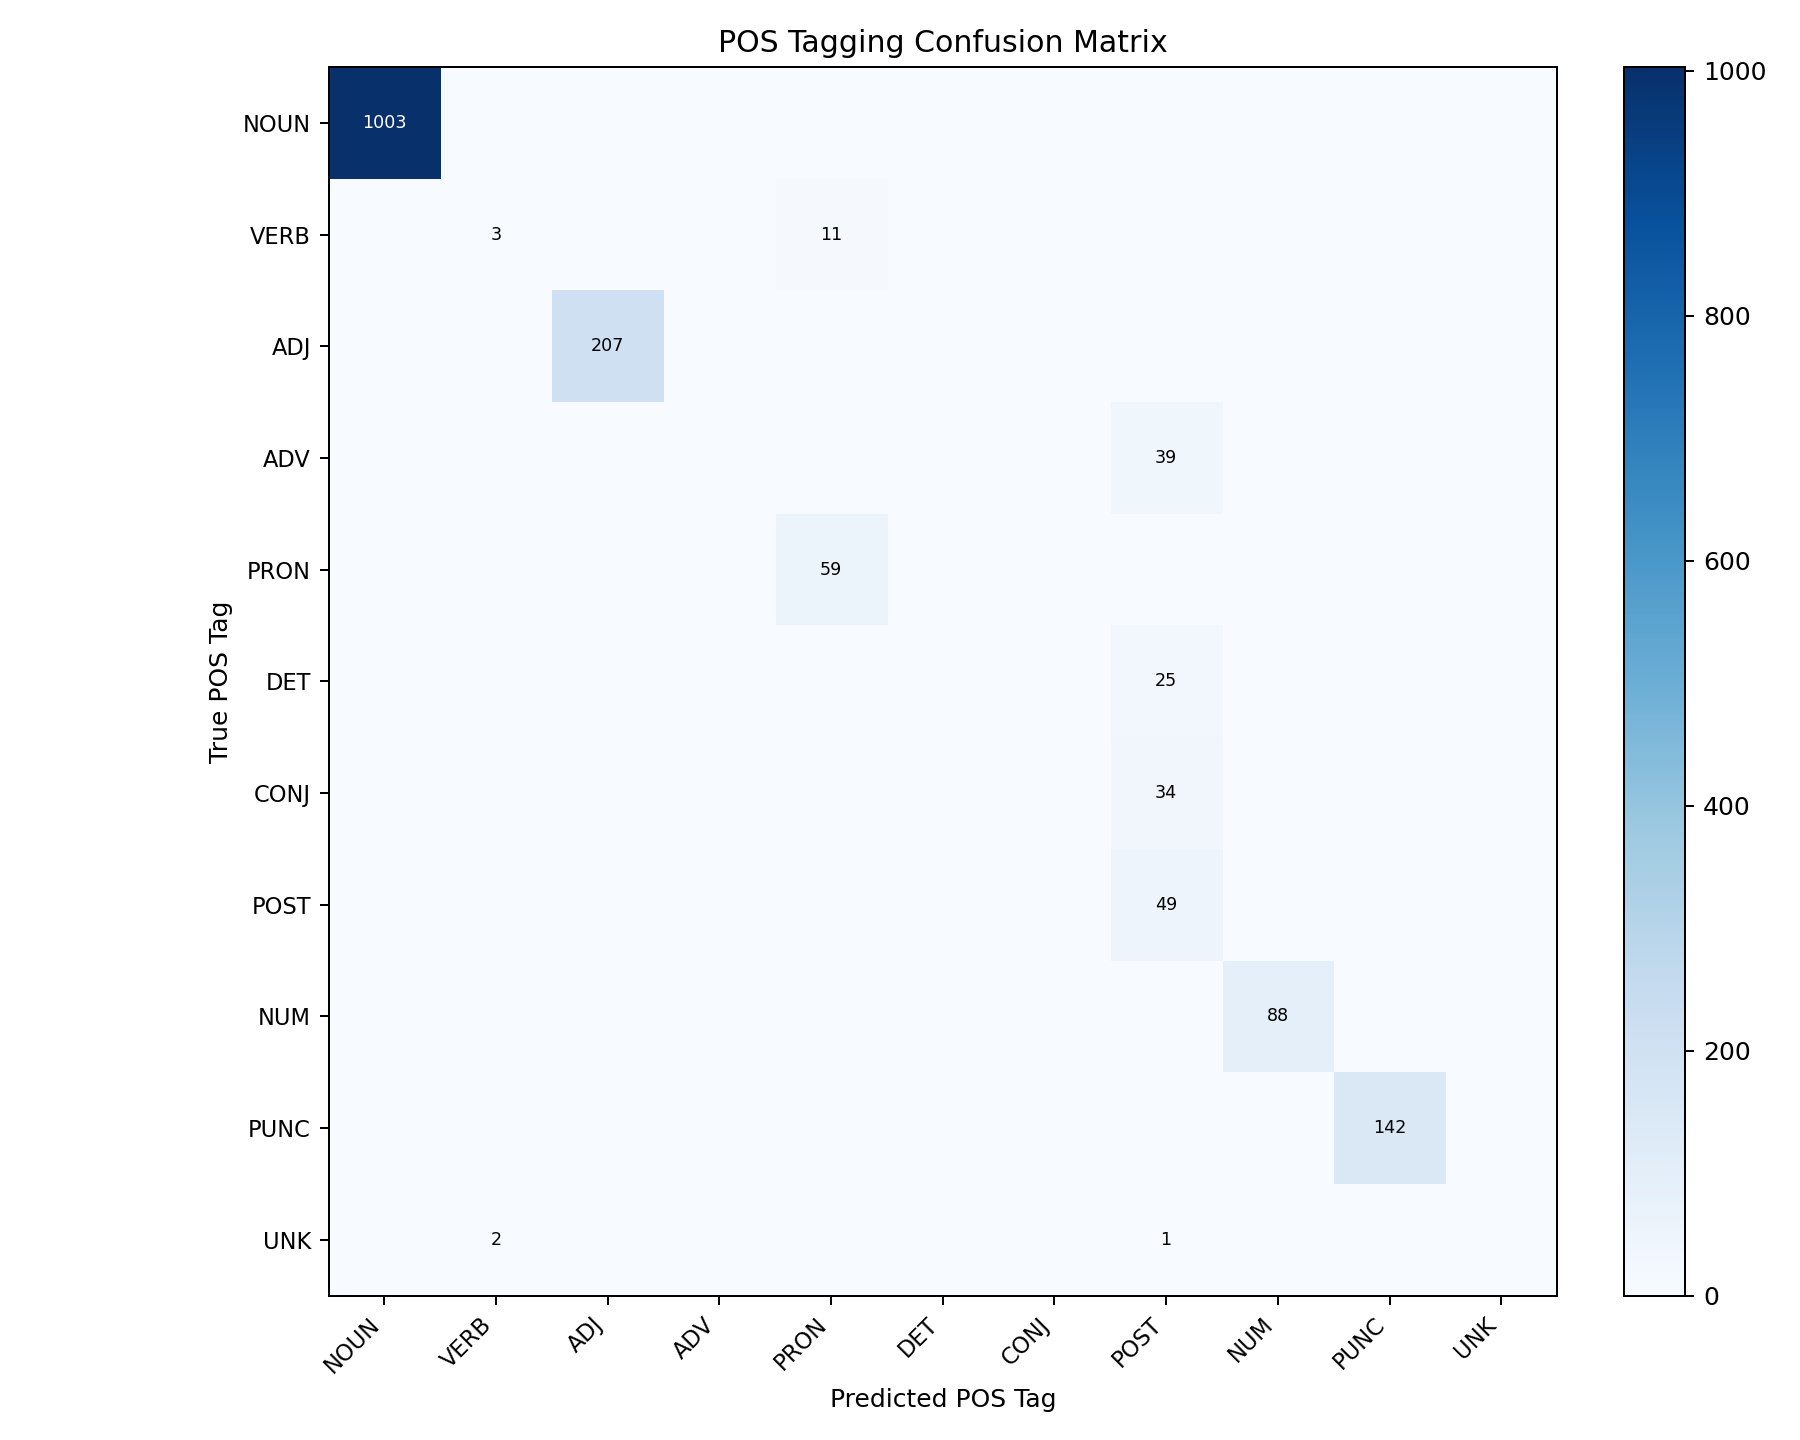
\includegraphics[width=0.65\linewidth]{Images to add/part2_pos_confusion_matrix.png}
    \caption{POS confusion matrix on the test set.}
\end{figure}

NER performance (conlleval-style entity metrics) is listed in Table~\ref{tab:ner_scores}.

\begin{table}[H]
\centering
\caption{NER entity-level results with CRF decoding}
\label{tab:ner_scores}
\begin{tabular}{lccc}
\toprule
Entity Type & Precision & Recall & F1 \\
\midrule
PER & 0.7303 & 0.4924 & 0.5882 \\
LOC & 0.9925 & 0.9779 & 0.9852 \\
ORG & 0.6149 & 0.8168 & 0.7016 \\
MISC & 0.9880 & 0.9960 & 0.9920 \\
Overall & 0.8532 & 0.8532 & 0.8532 \\
\bottomrule
\end{tabular}
\end{table}

CRF and no-CRF overall F1 differed in this run (0.8532 with CRF vs. 0.8022 without CRF).
Ablation experiments A1--A4 were completed; the summary is provided in Table~\ref{tab:ablations}.

\begin{table}[H]
\centering
\caption{Ablation study summary}
\label{tab:ablations}
\begin{tabular}{lcc}
\toprule
Ablation & POS Macro-F1 & NER Overall F1 \\
\midrule
A1 (Unidirectional LSTM) & 0.0684 & 0.0000 \\
A2 (No dropout) & 0.1746 & 0.4436 \\
A3 (Random embeddings) & 0.1833 & 0.4112 \\
A4 (Softmax instead of CRF) & -- & 0.3438 \\
\bottomrule
\end{tabular}
\end{table}

\section*{Part 3 Results: Transformer Encoder for Topic Classification}
A custom Transformer encoder (4 pre-LN blocks, 4 heads, sinusoidal PE, CLS token classifier) was trained with AdamW and cosine schedule.
Training and validation curves are shown in Figure~\ref{fig:part3_curves}.

\begin{figure}[H]
    \centering
    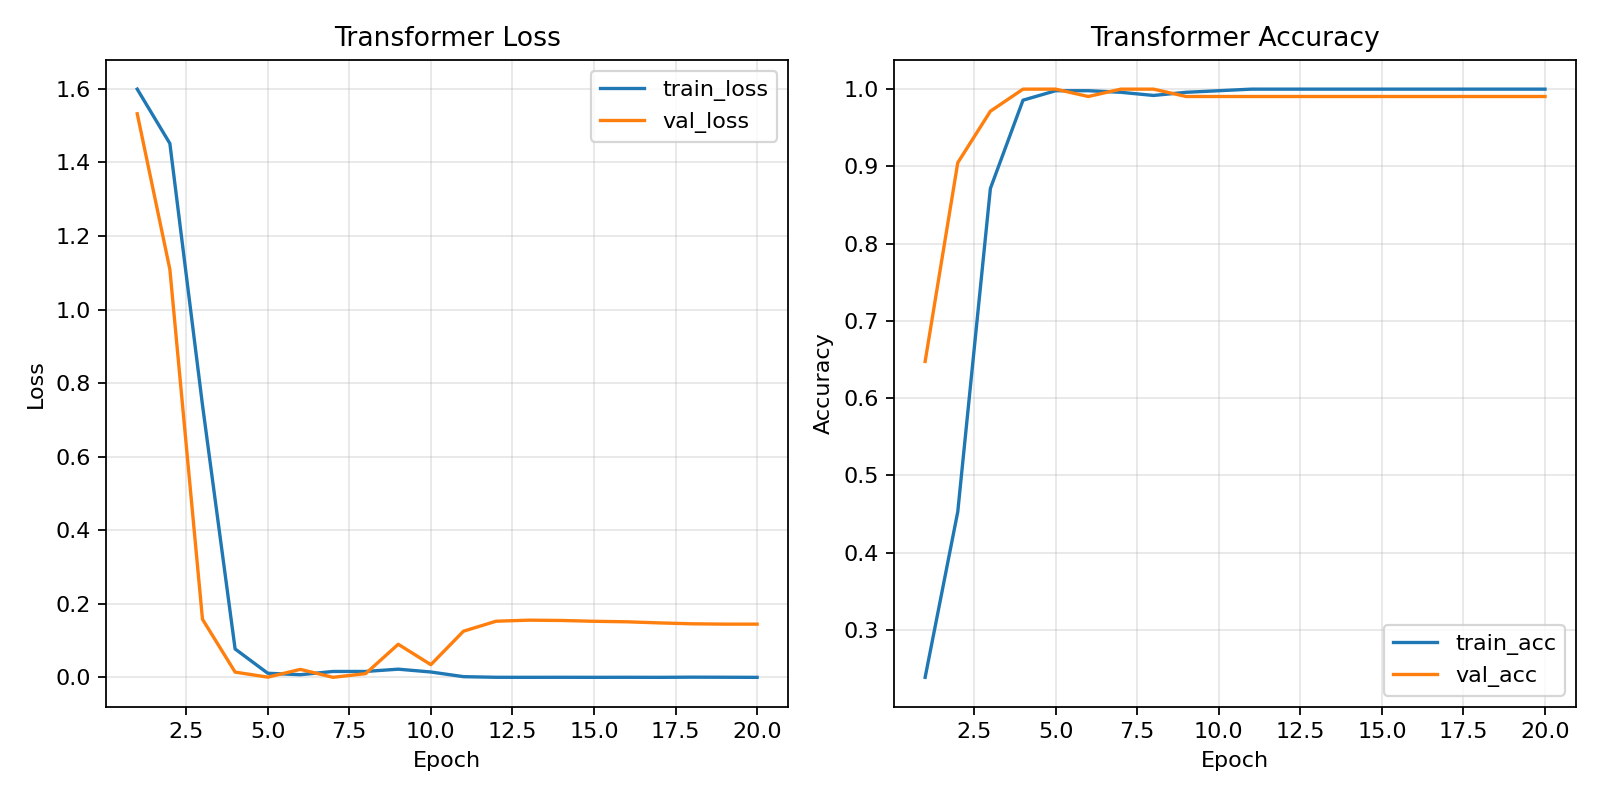
\includegraphics[width=0.9\linewidth]{Images to add/part3_transformer_curves.png}
    \caption{Transformer training and validation loss/accuracy curves.}
    \label{fig:part3_curves}
\end{figure}

Test-set classification performance in a leakage-checked rerun (seed $=101$, max length $=24$, epochs $=20$) was:
Transformer accuracy = 0.9905, macro-F1 = 0.9905.
The $5\times5$ confusion matrix is shown in Figure~\ref{fig:part3_cm}.

\begin{figure}[H]
    \centering
    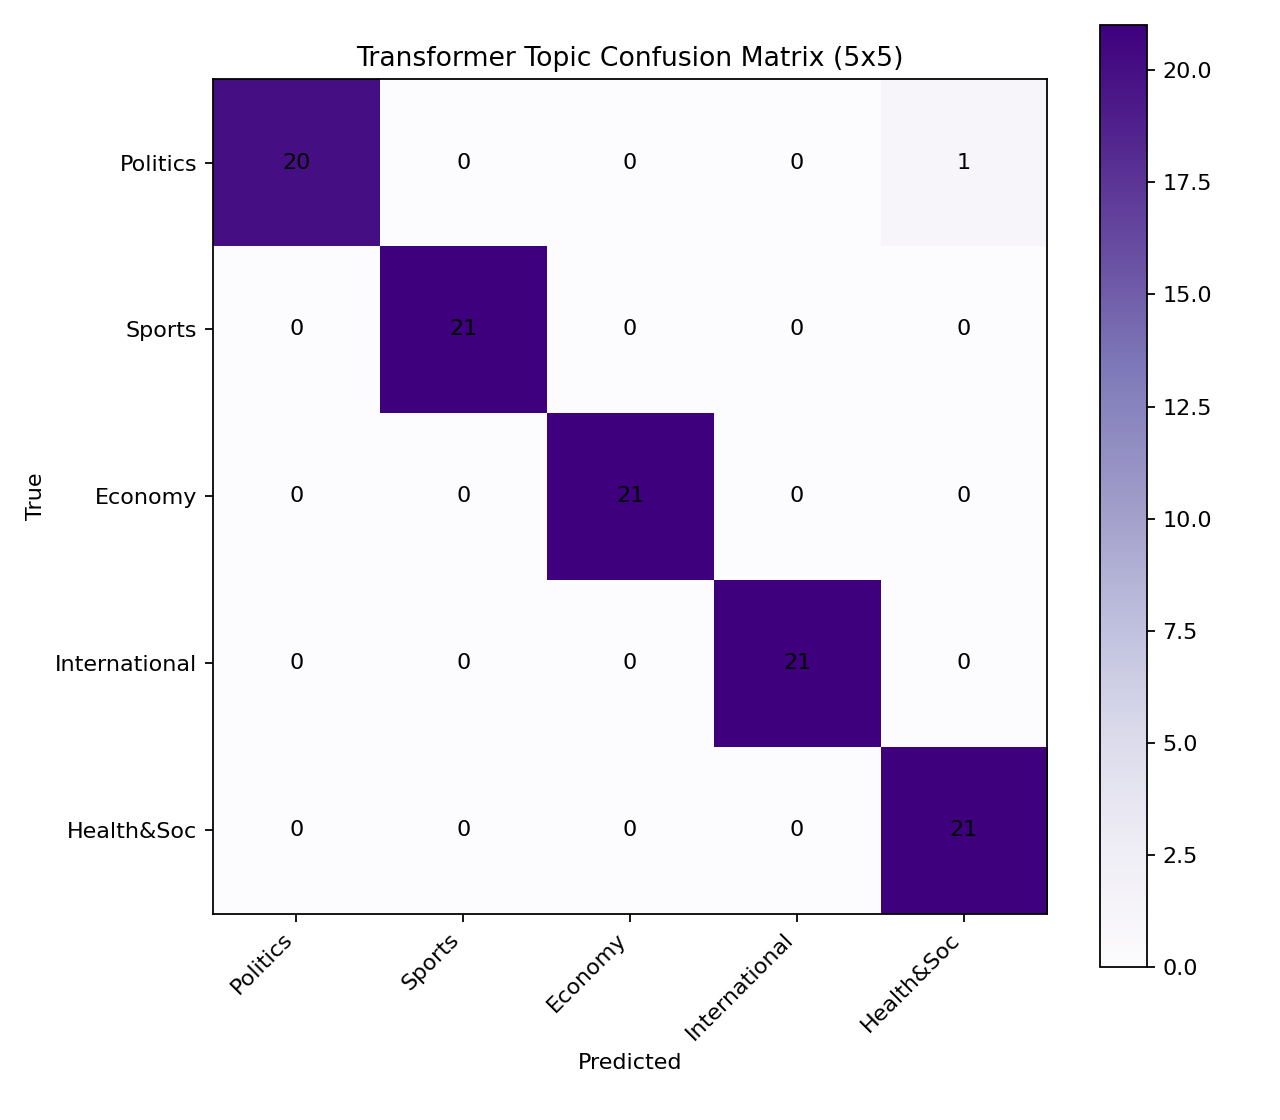
\includegraphics[width=0.72\linewidth]{Images to add/part3_topic_confusion_matrix.png}
    \caption{Transformer topic classification confusion matrix.}
    \label{fig:part3_cm}
\end{figure}

Attention analysis was performed using final-layer head maps for 3 correctly classified articles.
Representative heatmaps are shown in Figure~\ref{fig:attn}.

\begin{figure}[H]
    \centering
    \safeincludegraphics[width=0.48\linewidth]{Images to add/part3_attention_article1_head0.png}
    \safeincludegraphics[width=0.48\linewidth]{Images to add/part3_attention_article1_head1.png}
    \safeincludegraphics[width=0.48\linewidth]{Images to add/part3_attention_article2_head0.png}
    \safeincludegraphics[width=0.48\linewidth]{Images to add/part3_attention_article2_head1.png}
    \safeincludegraphics[width=0.48\linewidth]{Images to add/part3_attention_article3_head0.png}
    \safeincludegraphics[width=0.48\linewidth]{Images to add/part3_attention_article3_head1.png}
    \caption{Final-layer attention heatmaps (heads 0 and 1) for three correctly classified articles.}
    \label{fig:attn}
\end{figure}

\section*{BiLSTM vs. Transformer Comparison}
On the same stratified test split, the Transformer achieved 0.9905 accuracy and 0.9905 macro-F1.
The BiLSTM baseline achieved 0.9714 accuracy and 0.9716 macro-F1.
Therefore, the Transformer was higher by 0.0190 accuracy points in this run.
In terms of convergence, the Transformer reached peak validation accuracy at epoch 4.
The BiLSTM reached its best validation accuracy at epoch 3, so the BiLSTM converged in fewer epochs.
Average per-epoch training time was 7.38 seconds for the Transformer.
Average per-epoch training time was 3.50 seconds for the BiLSTM, which was slightly faster in wall-clock cost per epoch.
This runtime pattern is expected because attention layers add dense token-token interactions, while recurrent updates can be cheaper at the current sequence length and implementation settings.
The attention heatmaps show that specific topic-bearing tokens receive stronger influence on the final-layer pathways connected to the CLS representation.
These scores are still high because the corpus is balanced and topic cues are strong, but the rerun is non-perfect and includes concrete misclassifications.
For datasets with only 200--300 articles, the safer default choice is BiLSTM because it is typically more data-efficient and less sensitive to optimization hyperparameters.
The Transformer should be preferred at that scale only when strong regularization, careful learning-rate scheduling, and sufficient validation control are available.

\section*{Conclusion}
The assignment requirements were implemented end-to-end with reproducible code and generated artifacts.
Part 1 produced weighted lexical representations and Skip-gram embeddings with qualitative evaluation.
Part 2 delivered full POS/NER sequence labeling workflows with CRF and ablation studies.
Part 3 delivered a from-scratch Transformer encoder and comparative analysis with a BiLSTM baseline.
The accompanying notebook contains executed outputs for all required items, and this report summarizes the core quantitative and qualitative findings.

\end{document}
